% This is the Reed College LaTeX thesis template. Most of the work
% for the document class was done by Sam Noble (SN), as well as this
% template. Later comments etc. by Ben Salzberg (BTS). Additional
% restructuring and APA support by Jess Youngberg (JY).
% Your comments and suggestions are more than welcome; please email
% them to cus@reed.edu
%
% See http://web.reed.edu/cis/help/latex.html for help. There are a
% great bunch of help pages there, with notes on
% getting started, bibtex, etc. Go there and read it if you're not
% already familiar with LaTeX.
%
% Any line that starts with a percent symbol is a comment.
% They won't show up in the document, and are useful for notes
% to yourself and explaining commands.
% Commenting also removes a line from the document;
% very handy for troubleshooting problems. -BTS

% As far as I know, this follows the requirements laid out in
% the 2002-2003 Senior Handbook. Ask a librarian to check the
% document before binding. -SN

%%
%% Preamble
%%
% \documentclass{<something>} must begin each LaTeX document
\documentclass[12pt,twoside]{reedthesis}
% Packages are extensions to the basic LaTeX functions. Whatever you
% want to typeset, there is probably a package out there for it.
% Chemistry (chemtex), screenplays, you name it.
% Check out CTAN to see: http://www.ctan.org/
%%
\usepackage{graphicx,latexsym}
\usepackage[french]{babel} 
\usepackage{amsmath}
\usepackage{amssymb,amsthm}
\usepackage[dvipsnames]{xcolor} % tk: for more color
\usepackage{xcolor}
\usepackage{eso-pic}
\usepackage{longtable,booktabs,setspace}
\usepackage{chemarr} %% Useful for one reaction arrow, useless if you're not a chem major
\usepackage[hyphens]{url}
\usepackage{tikz}
\usetikzlibrary{calc}
\newcommand\HRule{\rule{\textwidth}{1pt}}
% Added by CII
\usepackage{hyperref}
\usepackage{lmodern}
\usepackage{float}
\floatplacement{figure}{H}
% End of CII addition
\usepackage{rotating}
\usepackage{upgreek} % tk : pour pouvoir utiliser le symbole µ droit (pas en itallic)



% Next line commented out by CII
%%% \usepackage{natbib}
% Comment out the natbib line above and uncomment the following two lines to use the new
% biblatex-chicago style, for Chicago A. Also make some changes at the end where the
% bibliography is included.
%\usepackage{biblatex-chicago}
%\bibliography{thesis}


% Added by CII (Thanks, Hadley!)
% Use ref for internal links
\renewcommand{\hyperref}[2][???]{\autoref{#1}}
\def\chapterautorefname{Chapter}
\def\sectionautorefname{Section}
\def\subsectionautorefname{Subsection}
% End of CII addition

% Added by CII
\usepackage{caption}
\captionsetup{width=5in}
% End of CII addition

% \usepackage{times} % other fonts are available like times, bookman, charter, palatino


% To pass between YAML and LaTeX the dollar signs are added by CII
\title{THÈSE}
\author{Thomas Karaouzene}
\labo{}
% The month and year that you submit your FINAL draft TO THE LIBRARY (May or December)
\date{31 octobre 2017}
\division{}
\advisor{Pierre Ray}
%If you have two advisors for some reason, you can use the following
% Uncommented out by CII
\altadvisor{Nicolas Thierry-Mieg}
% End of CII addition

%%% Remember to use the correct department!
\department{Ingénierie de la Santé, de la Cognition et Environnement (EDISCE)}
% if you're writing a thesis in an interdisciplinary major,
% uncomment the line below and change the text as appropriate.
% check the Senior Handbook if unsure.
%\thedivisionof{The Established Interdisciplinary Committee for}
% if you want the approval page to say "Approved for the Committee",
% uncomment the next line
%\approvedforthe{Committee}

% Added by CII
%%% Copied from knitr
%% maxwidth is the original width if it's less than linewidth
%% otherwise use linewidth (to make sure the graphics do not exceed the margin)
\makeatletter
\def\maxwidth{ %
  \ifdim\Gin@nat@width>\linewidth
    \linewidth
  \else
    \Gin@nat@width
  \fi
}
\makeatother

\renewcommand{\contentsname}{Table of Contents}
% End of CII addition

\setlength{\parskip}{0pt}

% Added by CII
  %\setlength{\parskip}{\baselineskip}
  \usepackage[parfill]{parskip}

\providecommand{\tightlist}{%
  \setlength{\itemsep}{0pt}\setlength{\parskip}{0pt}}

\Acknowledgements{

}

\Dedication{

}

\Preface{
This is an example of a thesis setup to use the reed thesis document
class (for LaTeX) and the R bookdown package, in general.
}

\Abstract{

}

	\usepackage{tikz}
% End of CII addition
%%
%% End Preamble
%%
%

\usepackage{amsthm}
\newtheorem{theorem}{Theorem}[section]
\newtheorem{lemma}{Lemma}[section]
\theoremstyle{definition}
\newtheorem{definition}{Definition}[section]
\newtheorem{corollary}{Corollary}[section]
\newtheorem{proposition}{Proposition}[section]
\theoremstyle{definition}
\newtheorem{example}{Example}[section]
\theoremstyle{remark}
\newtheorem*{remark}{Remark}
\begin{document}

% Everything below added by CII
      \maketitle
  
  \frontmatter % this stuff will be roman-numbered
  \pagestyle{empty} % this removes page numbers from the frontmatter

  
      \begin{preface}
      This is an example of a thesis setup to use the reed thesis document
      class (for LaTeX) and the R bookdown package, in general.
    \end{preface}
  
      \hypersetup{linkcolor=black}
    \setcounter{tocdepth}{3}
    \tableofcontents
  
      \listoftables
  
      \listoffigures
  
  
  
  \mainmatter % here the regular arabic numbering starts
  \pagestyle{fancyplain} % turns page numbering back on

  \chapter{Delete line 6 if you only have one
  advisor}\label{delete-line-6-if-you-only-have-one-advisor}
  
  \chapter*{Remerciements}\label{remerciements}
  \addcontentsline{toc}{chapter}{Remerciements}
  
  \chapter*{Résumé}\label{resume}
  \addcontentsline{toc}{chapter}{Résumé}
  
  \chapter{Introduction}\label{introInf}
  
  \chapter{Investigation génétique et physiologique de la
  globozoospermie}\label{globo}
  
  \chapter{Mise en place d'une stratégie pour l'analyse des données
  exomiques -- application en recherche
  clinique}\label{mise-en-place-dune-strategie-pour-lanalyse-des-donnees-exomiques-application-en-recherche-clinique}
  
  \section{Intro}\label{intro}
  
  Comme vu précédemment, l'émergence du séquençage haut débit, avec
  notamment le WGS et le WES, a révolutionné les méthodes de recherche
  dans le cadre d'étude phénotype-génotype en permettant de manière rapide
  et à moindre coup le séquençage de la quasi totalité des gènes humains.
  Les causes de plusieurs centaines de pathologies ont pu être identifiées
  grâce à ces technique depuis leur premier succès pubilié en 2010 (Ng et
  al., n.d.). Dès lors, l'analyse des données issues du séquençage est
  devenu la clef dans la réussite de ces études.
  
  Il existe de nombreux logiciels qui à partir des variants appelés
  effectuent les étapes d'annotation et de filtrage. C'est par exemple le
  cas d'Exomiser {[}TODO: insert ref and Exomiser describtion{]} ou encore
  de {[}TODO: insert at least one other soft{]}. La plupart de ces
  logiciels fonctionnent très bien, cependant tous prennent pour point de
  départ des variants appelés en amont. Ils ne contrôlent donc en aucune
  manière les étapes d'alignement et d'appel des variants. Or, comme il a
  été dit plus tôt, ces deux étapes constituent la bases de l'analyse
  {[}TODO insert ref{]} et les résultats
  
  Dans ce chapitre, je détaillerai les résultats de 4 articles dont je
  suis coauteur :
  
  \begin{enumerate}
  \def\labelenumi{\arabic{enumi}.}
  \tightlist
  \item
    \protect\hyperlink{famdnah1}{\textbf{Whole-exome sequencing of
    familial cases of multiple morphological abnormalities of the sperm
    flagella (MMAF) reveals new DNAH1 mutations}} : {[}todo{]}
  \item
    \protect\hyperlink{plcz}{\textbf{Homozygous mutation of PLCZ1 leads to
    defective human oocyte activation and infertility that is not rescued
    by the WW-binding protein PAWP}} : Dans cet article j'ai, comme
    précédemment, effectué l'integralité des analyses bioinformatiques des
    données d'exomes effectués sur deux frères infertiles présentant des
    échecs de fécondation.\\
  \item
    \protect\hyperlink{spink2}{\textbf{SPINK2 deficiency causes
    infertility by inducing sperm defects in heterozygotes and azoospermia
    in homozygotes}} : Dans cet article j'ai effectuer non seulement
    l'intégralité des analyses bioinformatiques des données d'exomes de
    deux frères infertiles présentant un phénotype d'azoospermie mais
    aussi séquencer en Sanger les séquences codantes du gène \emph{SPINK2}
    pour une parie des 611 individus analyser ainsi que contribué à
    l'extraction de l'ARN testiculaire des souris pour l'analyse
    fonctionelle du gène \emph{Spink2} sur le modèle murin.\\
  \item
    \protect\hyperlink{cohortemmah}{****} : {[}todo{]}
  \end{enumerate}
  
  \section{Résultats}\label{resultats}
  
  \subsection{Description de la
  pipeline}\label{description-de-la-pipeline}
  
  Notre pipeline d'analyse effectue l'ensemble des étapes allant de
  l'alignement des données jusqu'au filtrage des variants
  
  \begin{enumerate}
  \def\labelenumi{\arabic{enumi}.}
  \tightlist
  \item
    \textbf{L'alignement} : L'alignement des \emph{reads} le long du
    génome de référence est effectué par le logiciel MAGIC (Su et al.,
    \protect\hyperlink{ref-Su2014}{2014}). Celui-ci l'intégralité pour
    l'ensemble des analyses en aval l'ensemble des \emph{reads} dupliqués
    et / ou s'alignant à plusieurs zone du génome. Au cours de cette
    étape, MAGIC va produire également quatre comptages pour chaque
    position couverte du génome : R+, V+, R- et V- :
  
    \begin{enumerate}
    \def\labelenumii{\alph{enumii}.}
    \tightlist
    \item
      \textbf{R+ et R-} : Ces deux comptages correspondent au nombres de
      \emph{reads} \emph{forward} (+) et \emph{reverse} (-) sur lesquels
      est observé l'allere de \textbf{référence} (R) à une position
      donnée.\\
    \item
      \textbf{V+ et V-} : À l'inverse de R+ et R-, ces comptages
      correspondent au nombres de \emph{reads} \emph{forward} et
      \emph{reverse} sur lesquels est observé un allele de
      \textbf{variant} (V) à une position donnée.\\
    \end{enumerate}
  \item
    \textbf{L'appel des variants} : Comme nous l'avons vu plus
    \protect\hyperlink{varcall}{tôt}, il est fortement conseillé
    d'effectuer l'appel des variants en tenant compte de l'aligneur choisi
    (Nielsen, Paul, Albrechtsen, \& Song,
    \protect\hyperlink{ref-Nielsen2011}{2011}, M. A. DePristo et al.
    (\protect\hyperlink{ref-DePristo2011}{2011}), Lunter \& Goodson
    (\protect\hyperlink{ref-Lunter2011}{2011})). C'est pourquoi, nous
    avons conçu notre propre algorithme d'appel des variants spécialement
    conçu pour l'analyse des données de MAGIC. Ainsi, l'appel des variants
    sera directement basé sur les quatre comptages vu précédement. Tout
    d'abord, les positions ayant une couverture \textless{} 10 sur l'un
    des deux \emph{strands} sera considérée comme de faible qualité,
    celles aynant une couverture \textless{} 10 sur les deux
    \emph{strands} seront exclus. Ensuite pour chaque variant, des appels
    indépendant seront effectués pour chaque \emph{strand}. L'appel final
    sera une synthèse de ces deux appels où seul les cas où ces deux
    appels sont concordants seront considérés comme de bone qualité.\\
  \item
    \textbf{L'annotation} : Chaque variant retenu sera ensuite annoté tout
    d'abord par le logiciel \emph{variant effect predictor} (VEP) (W.
    McLaren et al., \protect\hyperlink{ref-McLaren2016}{2016}) qui nous
    indiquera pour chaque variant l'impact que celui-ci aura sur la
    séquence codante de l'ensemble des transcrits qu'il chevauche. Suite à
    cela nous ajoutons, lorsque celle-ci est disponible, la fréquence du
    variant dans les bases de données ExAC (Lek et al.,
    \protect\hyperlink{ref-Lek2016}{2016}), ESP600 {[}TODO{]} et
    1000Genomes {[}TODO{]} donnant ainsi une estimation de sa fréquence
    dans la population générale. De même, la particularité de cette
    pipeline est qu'elle conserve l'ensemble des variants identifiés dans
    les études effectués précédement permettant d'ajouter aux annotations
    la fréquences d'un variant chez les individus déjà séquencé et donc la
    fréquence d'un variant dans chaque phénotype étudié créant ainsi une
    base de données interne qui pourra servir de contrôle dans les études
    ulterieur.
  \item
    \textbf{Le filtrage des variants} : L'étape de filtrage est
    extremement importante si l'on souhaite analyser de manière efficace
    les données provenant de WES. C'est pourquoi elle occupe une place
    importante dans notre pipeline. L'intégralité des paramètres de cette
    étape peuvent être modifier par l'utilisateur de sorte à faire
    correspondre les critères de filtre aux bsoins de l'étude. Afin de
    rendre son utilisation le plus efficace possibe, nous avons souhaité
    définir des paramètres par défauts pertinent dans la plupart des étude
    de séquençage exomique de sorte que à moins que le contraire ne soit
    spécifié, seul les variants impactant les transcrits codant pour une
    protéine sont conservés. De même les variants synonymes ou affectant
    les séquences UTRs sont filtrés ainsi que les variants ayant une
    fréquence \(\ge\) 1\% dans les bases dans l'une des bases données
    (ExAC, ESP6500 ou 1KH). Aussi, pour un phénotype donné, l'ensemble des
    variants observés chez les individus étudiés présentant un phénotype
    différent sont de même enlevés de la liste finale.
  \end{enumerate}
  
  \subsection{Utilisation de la pipeline dans des cas familiaux
  :}\label{utilisation-de-la-pipeline-dans-des-cas-familiaux}
  
  \subsubsection{Description des familles}\label{description-des-familles}
  
  Dans cette partie, je me concentre sur l'analyse bioinformatique des
  résultat du séquençage exomique de treize individus provenant de quatre
  familles différentes (\textbf{Table : }\ref{tab:recapfam}) :
  
  \begin{table}
  
  \caption{\label{tab:recapfam}Tableau recapitulatif des familles séquencées}
  \centering
  \begin{tabular}[t]{l|r|l|r|l|l}
  \hline
  Familly & Individuals & Phenotype & Year & Plateform & Place\\
  \hline
  Az & 2 & Azoospermia & 2012 & Illumina HiSeq2000 & Mount Sinai Institut\\
  \hline
  FF & 2 & Fertilization failure & 2014 & Illumina HiSeq2000 & Genoscope (Evry)\\
  \hline
  MMAF1 & 2 & MMAF & 2014 & Illumina HiSeq2000 & Genoscope (Evry)\\
  \hline
  MMAF2 & 2 & MMAF & 2014 & Illumina HiSeq2000 & Genoscope (Evry)\\
  \hline
  MMAF3 & 2 & MMAF & 2014 & Illumina HiSeq2000 & Genoscope (Evry)\\
  \hline
  MMAF4 & 3 & MMAF & 2014 & Illumina HiSeq2000 & Genoscope (Evry)\\
  \hline
  \end{tabular}
  \end{table}
  
  \subsubsection{Resultats des exomes}\label{resultats-des-exomes}
  
  Pour l'ensemble des individus de ces quatre familles nous avons appliqué
  notre pipeline d'analyse de sorte à obtenir pour chaque patient une
  liste de SNV et d'indel avec leur génotype associé (\textbf{Figure :
  }\ref{fig:resvarcall}). Afin de connaitre l'impact de ces variants et
  ainsi nous concentrer sur ceux ayant la plus forte probabilité d'être
  responsables du phénotype nous les avons annoté grâce au logiciel VEP.
  Les différentes annotations apportées nous ont tout d'abord permis de
  filtrer l'intégralité des variants chevauchant un transcrit annoté
  \emph{nonsense-mediated decay} (NMD). En effet, ce mécanisme a pour but
  de controler la qualité des ARNm cellulaires chez les eucaryotes (Y.-F.
  Chang, Imam, \& Wilkinson, \protect\hyperlink{ref-Chang2007}{2007}) en
  éliminant les ARNm qui comportent un codon stop prématuré (Baker \&
  Parker, \protect\hyperlink{ref-Baker2004}{2004}), pouvant être le
  résultat d'une erreur de transcription, d'une mutation ou encore d'une
  erreur d'épissage. Cette première étape de filtre permet à elle seule de
  filtrer systematiquement les variants de 2587 à 3212 transcrits en
  fonction des individus soit, entre 7261 et 10872 variants différent par
  individus (\textbf{Figure : }\ref{fig:nmdtranscripts}).
  
  \begin{figure}
  
  {\centering \includegraphics{thesis_files/figure-latex/nmdtranscripts-1} 
  
  }
  
  \caption[Nombre de transcrits et variants filtrés car ils sont annotés NMD]{Nombre de transcrits et variants filtrés car ils sont annotés NMD : Chaque point représente un individu séquencé, la couleur et la forme du point dépend de la famille d'origine de l'individu}\label{fig:nmdtranscripts}
  \end{figure}
  
  Parmi ces variants, nous avons filtrés l'ensemble de ceux chevauchant
  uniquement des transcrits annotés \emph{NMD} (\emph{non sense mediated
  decay}) par VEP qui représentent entre XXX et YYY (TODO)\% des
  transcrits afin de nous concentrer sur les variants ayant la plus forte
  probabilité d'avoir un effet sur une protéine. Chacun de ces variants a
  été confronté à une liste de variants homozygotes observés sur les
  individus sains ou présentant un phénotype différent des patients
  étudiés de notre bases de données interne (\textbf{Figure :
  }\ref{fig:plotsamplectrl}). Cette
  
  \begin{figure}
  
  {\centering \includegraphics{thesis_files/figure-latex/resvarcall-1} 
  
  }
  
  \caption[Comptage des SNVs et indels retrouvés par patients avec leur génotypes associés]{Comptage des SNVs et indels retrouvés par patients avec leur génotypes associés}\label{fig:resvarcall}
  \end{figure}
  
  \begin{figure}
  
  {\centering \includegraphics{thesis_files/figure-latex/plotsamplectrl-1} 
  
  }
  
  \caption[Nombre d'individus dans chaque famille et taille de la cohorte contrôle utilisée dans l'analyse]{Nombre d'individus dans chaque famille et taille de la cohorte contrôle utilisée dans l'analyse : Le diagramme en barre du haut montre la taille des cohorte contrôle utilisée pour chaque famille. Un individus "contrôle" peut être soit sain ou ne pas présenter le même phénotype que les individus de la famille analysée. Le diagramme du bas présente le nombre d'individus analysées dans chacune des familles. Chaque couleur correspond à une famille.}\label{fig:plotsamplectrl}
  \end{figure}
  
  \begin{figure}
  
  {\centering \includegraphics{thesis_files/figure-latex/remaininggenes-1} 
  
  }
  
  \caption[Nombre de gènes passant l'ensemble des filtres par famille]{Nombre de gènes passant l'ensemble des filtres par famille}\label{fig:remaininggenes}
  \end{figure}
  
  \hypertarget{cohortemmah}{\subsubsection{Etude d'une large cohorte de
  patients MMAF}\label{cohortemmah}}
  
  \begin{center}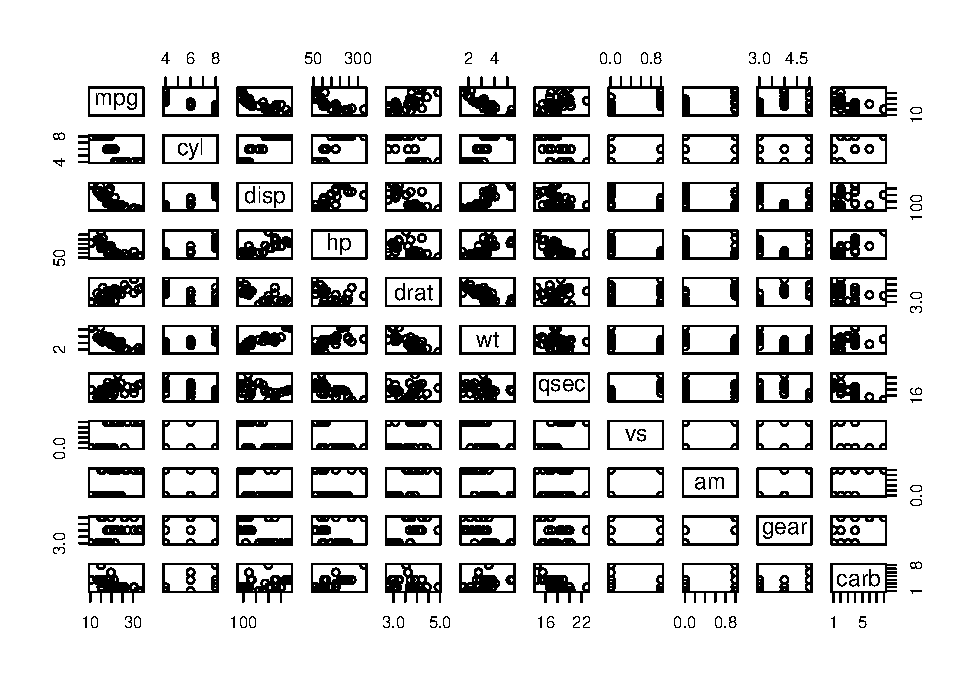
\includegraphics{thesis_files/figure-latex/aaa-1} \end{center}
  
  \begin{center}\includegraphics{thesis_files/figure-latex/aaa-2} \end{center}
  
  \begin{center}\includegraphics{thesis_files/figure-latex/aaa-3} \end{center}
  
  \begin{center}\includegraphics{thesis_files/figure-latex/aaa-4} \end{center}
  
  \begin{center}\includegraphics{thesis_files/figure-latex/aaa-5} \end{center}
  
  \chapter{MutaScript}\label{mutascript}
  
  \chapter*{Conclusion}\label{conclusion}
  \addcontentsline{toc}{chapter}{Conclusion}
  
  \chapter{The First Appendix}\label{the-first-appendix}
  
  \chapter*{References}\label{references}
  \addcontentsline{toc}{chapter}{References}
  
  \hypertarget{refs}{}
  \hypertarget{ref-Baker2004}{}
  Baker, K. E., \& Parker, R. (2004). Nonsense-mediated mRNA decay:
  terminating erroneous gene expression. \emph{Current Opinion in Cell
  Biology}, \emph{16}(3), 293--9.
  \url{http://doi.org/10.1016/j.ceb.2004.03.003}
  
  \hypertarget{ref-Chang2007}{}
  Chang, Y.-F., Imam, J. S., \& Wilkinson, M. F. (2007). The
  Nonsense-Mediated Decay RNA Surveillance Pathway. \emph{Annual Review of
  Biochemistry}, \emph{76}(1), 51--74.
  \url{http://doi.org/10.1146/annurev.biochem.76.050106.093909}
  
  \hypertarget{ref-DePristo2011}{}
  DePristo, M. A., Banks, E., Poplin, R., Garimella, K. V., Maguire, J.
  R., Hartl, C., \ldots{} Pritchard, E. (2011). A framework for variation
  discovery and genotyping using next-generation DNA sequencing data.
  \emph{Nature Genetics}, \emph{43}(5), 491--498.
  \url{http://doi.org/10.1038/ng.806}
  
  \hypertarget{ref-Lek2016}{}
  Lek, M., Karczewski, K. J., Minikel, E. V., Samocha, K. E., Banks, E.,
  Fennell, T., \ldots{} Exome Aggregation Consortium, D. G. (2016).
  Analysis of protein-coding genetic variation in 60,706 humans.
  \emph{Nature}, \emph{536}(7616), 285--91.
  \url{http://doi.org/10.1038/nature19057}
  
  \hypertarget{ref-Lunter2011}{}
  Lunter, G., \& Goodson, M. (2011). Stampy: A statistical algorithm for
  sensitive and fast mapping of Illumina sequence reads. \emph{Genome
  Research}, \emph{21}(6), 936--939.
  \url{http://doi.org/10.1101/gr.111120.110}
  
  \hypertarget{ref-McLaren2016}{}
  McLaren, W., Gil, L., Hunt, S. E., Riat, H. S., Ritchie, G. R. S.,
  Thormann, A., \ldots{} Cunningham, F. (2016). The Ensembl Variant Effect
  Predictor. \emph{Genome Biology}, \emph{17}(1), 122.
  \url{http://doi.org/10.1186/s13059-016-0974-4}
  
  \hypertarget{ref-Ng}{}
  Ng, S. B., Buckingham, K. J., Lee, C., Bigham, A. W., Tabor, H. K.,
  Dent, K. M., \ldots{} Bamshad, M. J. (n.d.). Exome sequencing identifies
  the cause of a Mendelian disorder. \url{http://doi.org/10.1038/ng.499}
  
  \hypertarget{ref-Nielsen2011}{}
  Nielsen, R., Paul, J. S., Albrechtsen, A., \& Song, Y. S. (2011).
  Genotype and SNP calling from next-generation sequencing data.
  \emph{Nature Reviews. Genetics}, \emph{12}(6), 443--51.
  \url{http://doi.org/10.1038/nrg2986}
  
  \hypertarget{ref-Su2014}{}
  Su, Z., Łabaj, P. P., Li, S. S., Thierry-Mieg, J., Thierry-Mieg, D.,
  Shi, W., \ldots{} Shi, L. (2014). A comprehensive assessment of RNA-seq
  accuracy, reproducibility and information content by the Sequencing
  Quality Control Consortium. \emph{Nature Biotechnology}, \emph{32}(9),
  903--14. \url{http://doi.org/10.1038/nbt.2957}


  % Index?

\end{document}

